
\section{Splin\label{sec:Splines}}

Polinom oskulasi memiliki kegunaan terbatas dalam aplikasi yang mengharuskan
suatu kurva melalui sejumlah besar titik. Dan jumlah besar mungkin
hanya berarti sekitar \textit{setengah lusin}. Perhatikan himpunan
titik yang tampak biasa berikut ini.

\begin{center}
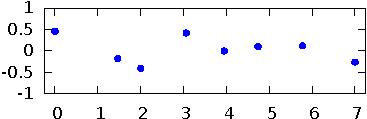
\includegraphics[width=7.5cm]{figures/generalizedSplines01}
\par\end{center}

\noindent Mudah untuk membayangkan suatu fungsi yang tampak sama sederhananya
dan melalui titik ini, tetapi mencari fungsi tersebut ternyata sedikit
menantang. Polinom interpolasi berderajat terendah berosilasi terlalu
lebar.

\begin{center}
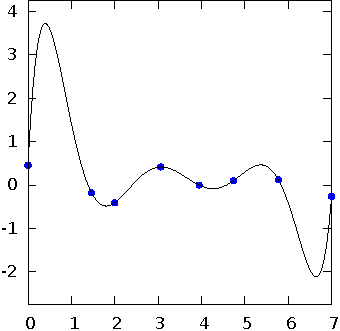
\includegraphics[width=7.5cm]{figures/generalizedSplines02}
\par\end{center}

\noindent Ini merupakan masalah umum pada polinom interpolasi berderajat
tinggi. Tidak ada kendali terhadap osilasinya, dan osilasi tersebut
biasanya tidak diinginkan. Osilasinya dapat diredam sampai tingkat
tertentu dengan mencari polinom oskulasi yang melalui titik-titik
ini dengan, misalnya, turunan pertama sebesar $0$ pada $0$ dan sebesar
$-\frac{1}{2}$ pada titik ketujuh dari kiri (titik yang koordinat
$x$-nya berada di antara 5 dan 6).

\begin{center}
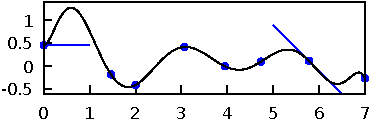
\includegraphics[width=7.5cm]{figures/generalizedSplines03}
\par\end{center}

\noindent Itu lebih baik, tetapi masih belum sepenuhnya memuaskan.
Menetapkan turunan pertama pada dua titik semata-mata untuk mengurangi
osilasi juga agak sewenang-wenang---lebih baik membiarkan sifat masalah
yang menentukan. Osilasi pada percobaan sebelumnya membuat hasilnya
terlalu khas dan menarik bagi himpunan titik hambar yang menjadi titik
awal kita. Cara yang sepantasnya sederhana untuk menginterpolasi data
tersebut adalah menghubungkan titik-titik berurutan dengan ruas garis.

\begin{center}
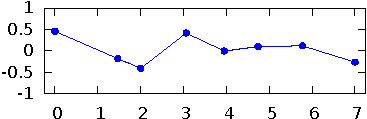
\includegraphics[width=7.5cm]{figures/generalizedSplines04}
\par\end{center}

\noindent Ini membentuk apa yang dikenal sebagai interpolasi linear
sepotong-sepotong dari himpunan data tersebut. Jenis grafik ini sering
terlihat di media massa. Namun, banyak aplikasi, terutama yang berasal
dari bidang teknik, memerlukan suatu tingkat kehalusan. Menghubungkan
setiap tiga titik berurutan dengan fungsi kuadratik dapat membantu.

\begin{center}
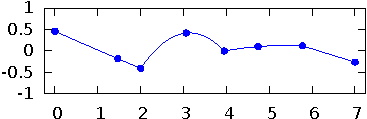
\includegraphics[width=7.5cm]{figures/generalizedSplines05}
\par\end{center}

\noindent Hal itu menjamin kehalusan pada tiga titik, tetapi fungsi
tersebut masih belum terdiferensialkan pada titik-titik yang dipakai
bersama oleh fungsi kuadratik berurutan. Selain itu, menggunakan tiga
titik pertama untuk fungsi kuadratik pertama (yang tampak linear bagi
mata telanjang), titik ketiga sampai kelima untuk fungsi kuadratik
kedua, dan titik kelima sampai ketujuh untuk fungsi kuadratik ketiga
(yang juga tampak linear bagi mata telanjang) hanya menyisakan titik
ketujuh dan kedelapan untuk fungsi yang semestinya merupakan fungsi
kuadratik keempat. Namun, karena hanya ada dua titik, sebagai gantinya
digunakan ruas garis. Solusi yang lebih halus adalah memastikan bahwa
turunan pertama fungsi kuadratik berurutan cocok pada titik bersama.
Dengan gagasan ini, masuk akal untuk mencocokkan hanya dua titik dengan
setiap parabola, sehingga tersisa satu koefisien (dari tiga pada setiap
fungsi kuadratik) untuk mencocokkan turunan fungsi kuadratik tetangganya.

\begin{center}
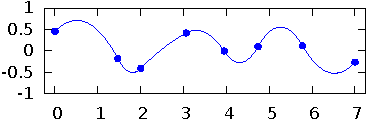
\includegraphics[width=7.5cm]{figures/generalizedSplines06}
\par\end{center}

\noindent Itu lebih baik! Fungsi parabola sepotong-sepotong ini memiliki
turunan pertama yang kontinu, tetapi masih ada sesuatu yang sewenang-wenang.
Ketujuh parabola itu secara keseluruhan memiliki 21 koefisien. Membuat
setiap parabola melalui dua titik memberikan 14 syarat pada koefisien-koefisien
tersebut. Mencocokkan turunan pertama parabola-parabola yang berdampingan
pada titik bersama memberikan 6 syarat lagi, satu pada masing-masing
dari 6 titik interior. Hal ini menyisakan satu koefisien ``bebas''.
Menetapkan satu syarat terakhir tampak agak sewenang-wenang, dan memang
demikian. Grafik menunjukkan hasil ketika turunan pada $0$ ditetapkan
menjadi $1$. Perhatikan bahwa tidak ada kendali terhadap turunan
di ujung kanan. Selain sifatnya yang sewenang-wenang, ketidaksimetrian
ini mengganggu. Andaikan kita memiliki satu derajat kebebasan lagi...

\subsection{Polinom sepotong-sepotong}

Suatu fungsi yang didefinisikan sepotong-sepotong dan semua potongannya
berupa polinom disebut polinom sepotong-sepotong. Bentuknya adalah
\[
p(x)=\begin{cases}
p_{1}(x), & x\in[x_{0},x_{1}]\\
p_{2}(x), & x\in(x_{1},x_{2}]\\
 & \vdots\\
p_{n}(x) & x\in(x_{n-1},x_{n}]
\end{cases}
\]
dengan $p_{i}(x)$ merupakan polinom untuk setiap $i=1,2,\ldots,n$
dan $x_{0}<x_{1}<\cdots<x_{n}$; atau suatu varian yang membuat $p(x_{j})$
didefinisikan oleh tepat satu dari $p_{i}$. Jika setiap $p_{i}$
merupakan fungsi linear, $p$ disebut linear sepotong-sepotong. Jika
setiap $p_{i}$ merupakan fungsi kuadratik, $p$ disebut kuadratik
sepotong-sepotong. Jika setiap $p_{i}$ merupakan fungsi kubik, $p$
disebut kubik sepotong-sepotong. Demikian seterusnya. Contoh fungsi
linear sepotong-sepotong dan kuadratik sepotong-sepotong terdapat
pada pendahuluan bagian ini.

\subsection{Splin}

Definisi polinom sepotong-sepotong sama sekali tidak mengharuskan
fungsi tersebut terdiferensialkan atau bahkan kontinu. Fungsi berikut
merupakan polinom sepotong-sepotong.

\begin{center}
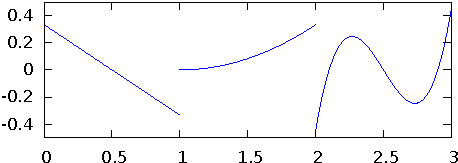
\includegraphics[width=7.5cm]{figures/generalizedSplines07}
\par\end{center}

\noindent Namun, sebagian besar aplikasi polinom sepotong-sepotong
memerlukan kekontinuan atau keterdiferensialan. Setiap polinom sepotong-sepotong
dengan sedikitnya satu turunan kontinu disebut splin. Titik-titik
yang memisahkan potongan-potongan yang berdampingan, yaitu $x_{j}$,
untuk $j=1,2,\ldots,n-1$, disebut simpul atau sambungan.

Grafik terakhir pada pendahuluan bagian ini memperlihatkan splin kuadratik.
Setiap potongan fungsi sepotong-sepotong tersebut merupakan fungsi
kuadratik, dan fungsi-fungsi kuadratik itu dipilih agar turunannya
cocok pada sambungan. Namun, seperti yang telah dinyatakan di sana,
kita perlu memberikan satu syarat yang tidak alami---turunan pada
titik ujung kiri. Syarat itu dapat berupa turunan pada titik mana
pun, atau bahkan turunan kedua pada salah satu titik. Dalam arti yang
sangat nyata, pilihan tersebut sewenang-wenang. Pilihan itu tidak
ditentukan secara alami oleh masalah yang dihadapi. Akibatnya, terdapat
suatu keluarga solusi untuk masalah menghubungkan delapan titik tersebut
dengan fungsi kuadratik sepotong-sepotong yang terdiferensialkan secara
kontinu.

\subsection{Splin kubik}

Splin yang paling umum digunakan adalah splin kubik. Seperti pada
splin kuadratik, splin kubik dihitung dengan mencocokkan turunan pada
sambungan. Bahkan, himpunan fungsi kubik memiliki cukup banyak koefisien
sehingga turunan pertama maupun kedua dapat dicocokkan. Namun, perhatikan
bahwa menurut definisi splin kita, pencocokan turunan pertama dan
kedua pada sambungan tidak sepenuhnya diperlukan. Sumber lain akan
memberikan definisi splin yang lebih ketat, yang mengharuskan pencocokan
kedua turunan tersebut. Sebagai konvensi, kita berfokus pada splin
seperti itu.

Splin kubik yang harus menginterpolasi $n+1$ titik memiliki $n-1$
sambungan dan $n$ potongan. Oleh karena itu, himpunan fungsi kubik
tersebut memiliki $4n$ koefisien. Mengharuskan setiap fungsi kubik
melalui $2$ titik menghasilkan $2n$ syarat pada koefisien. Mengharuskan
turunan pertama cocok pada sambungan memberikan $n-1$ syarat lagi.
Mengharuskan turunan kedua cocok pada sambungan memberikan tambahan
$n-1$ syarat, sehingga jumlah keseluruhannya adalah $4n-2$ syarat.
Hal ini menyisakan $2$ koefisien ``bebas''. Secara matematis, kita
memiliki suatu keluarga splin dengan dua derajat kebebasan. Untuk
memperoleh suatu splin tertentu, kita perlu memberlakukan dua syarat
lagi pada koefisien. Syarat-syarat ini dapat berupa turunan pertama,
kedua, atau ketiga pada dua simpul; turunan pertama dan kedua pada
satu simpul; atau kombinasi lain dari dua persyaratan turunan.

Mungkin dengan berpedoman pada pengetahuan tentang splin juru gambar,
konvensi mengarahkan kita untuk menetapkan syarat titik ujung. Artinya,
kita mensyaratkan sesuatu mengenai suatu turunan di $x_{0}$ dan di
$x_{n}$. Menentukan turunan pertama serupa dengan mengarahkan splin
juru gambar ke arah tertentu pada kedua ujungnya. Menetapkan turunan
kedua sama dengan $0$ serupa dengan membiarkan kedua ujung splin
juru gambar menunjuk bebas ke arah mana pun yang dibawa oleh hukum
fisika. Model splin juru gambar ini tidak terlalu akurat, tetapi memberikan
motivasi. 

Splin kubik yang turunan pertamanya ditentukan pada kedua titik ujung
disebut splin terapit. Splin kubik yang turunan keduanya ditetapkan
sama dengan nol pada kedua titik ujung disebut splin alami atau bebas.
Bentuk hibrida yang turunan pertamanya ditentukan pada satu ujung
dan turunan keduanya ditetapkan nol pada ujung lainnya tidak memiliki
nama khusus. Secara tepat, kita memiliki definisi berikut.

Misalkan $(x_{0},y_{0}),(x_{1},y_{1}),\ldots,(x_{n},y_{n})$ adalah
$n+1$ titik dengan $x_{0}<x_{1}<\cdots<x_{n}$, dan misalkan $S_{i}(x)=a_{i}+b_{i}(x-x_{i})+c_{i}(x-x_{i})^{2}+d_{i}(x-x_{i})^{3}$
untuk $i=1,2,\ldots,n$. Maka $S$, yang didefinisikan oleh 
\[
S(x)=\begin{cases}
S_{1}(x), & x\in[x_{0},x_{1}]\\
S_{2}(x), & x\in[x_{1},x_{2}]\\
 & \vdots\\
S_{n}(x), & x\in[x_{n-1},x_{n}]
\end{cases},
\]
merupakan splin kubik jika memenuhi tiga syarat berikut.
\begin{enumerate}
\item $S_{i}(x_{i-1})=y_{i-1}$ dan $S_{i}(x_{i})=y_{i}$ untuk $i=1,2,\ldots,n$
(interpolasi)
\item $S_{i}'(x_{i})=S_{i+1}'(x_{i})$ dan $S_{i}''(x_{i})=S_{i+1}''(x_{i})$
untuk $i=1,2,\ldots,n-1$ (pencocokan turunan)
\item Salah satu dari syarat berikut dipenuhi (syarat titik ujung)

\begin{enumerate}
\item \label{enu:naturalSpline}$S_{1}''(x_{0})=S_{n}''(x_{n})=0$
\item \label{enu:clampedSpline}$S_{1}'(x_{0})=m_{0}$ dan $S_{n}'(x_{n})=m_{n}$
untuk suatu $m_{0}$ dan $m_{n}$
\item \label{enu:mixed}$S_{1}'(x_{0})=m_{0}$ untuk suatu $m_{0}$ dan
$S_{n}''(x_{n})=0$
\item $S_{1}''(x_{0})=0$ dan $S_{n}'(x_{n})=m_{n}$ untuk suatu $m_{n}$
\end{enumerate}
\end{enumerate}
Jika kondisi titik ujung \ref{enu:naturalSpline} dipenuhi, $S$ disebut
splin bebas atau splin alami. Jika kondisi titik ujung \ref{enu:clampedSpline}
dipenuhi, $S$ disebut splin terapit.

Splin (kubik) alami yang melalui delapan titik yang disajikan dalam
pendahuluan bagian ini tampak seperti berikut. 

\begin{center}
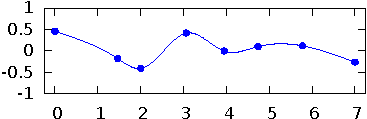
\includegraphics[width=7.5cm]{figures/generalizedSplines08}
\par\end{center}

\noindent Akhirnya, sebuah fungsi yang sama tidak istimewanya dengan
himpunan datanya! Bagaimana cara menghitungnya, Anda bertanya? Jawaban
singkatnya: 28 persamaan simultan yang dihasilkan dari definisi splin
kubik alami diselesaikan. Penyelesaiannya memberikan koefisien $a_{i},b_{i},c_{i},d_{i}$,
$i=1,2,\ldots,7$.

\subsubsection{Menyusun persamaan}

Jawaban panjangnya memang agak lebih panjang untuk diuraikan, tetapi
sebenarnya hanya berbeda dari versi singkat dalam tingkat kerinciannya.
Sebagai langkah awal, syarat $S_{i}(x_{i})=y_{i}$ langsung memberi
kita nilai bagi $n$ koefisien:
\[
S_{i}(x_{i})=a_{i}=y_{i}.
\]
Syarat $S_{i}(x_{i-1})=y_{i-1}$ memberi kita $n$ persamaan
\begin{equation}
S_{i}(x_{i-1})=y_{i}+b_{i}(x_{i-1}-x_{i})+c_{i}(x_{i-1}-x_{i})^{2}+d_{i}(x_{i-1}-x_{i})^{3}=y_{i-1}\label{eq:interpolationRequirement}
\end{equation}
untuk $i=1,2,\ldots,n$. Masing-masing syarat turunan memberi kita
$n-1$ persamaan:
\begin{eqnarray}
S_{i}'(x_{i})=S_{i+1}'(x_{i}) & \Rightarrow & b_{i}=b_{i+1}+2c_{i+1}(x_{i}-x_{i+1})+3d_{i+1}(x_{i}-x_{i+1})^{2}\label{eq:firstDerivativeRequirement}\\
S_{i}''(x_{i})=S_{i+1}''(x_{i}) & \Rightarrow & 2c_{i}=2c_{i+1}+6d_{i+1}(x_{i}-x_{i+1})\label{eq:secondDerivative Requirement}
\end{eqnarray}
untuk $i=1,2,\ldots,n-1$. Terakhir, kondisi titik ujung memberi kita
dua persamaan
\begin{eqnarray}
S_{1}''(x_{0}) & = & 2c_{1}+6d_{1}(x_{0}-x_{1})=0\label{eq:freeLeftEndpoint}\\
S_{n}''(x_{n}) & = & 2c_{n}=0.\label{eq:freeRightEndpoint}
\end{eqnarray}
Tanpa banyak kesulitan, kita memperoleh nilai $a_{i}$ dan $c_{n}$.
Sisa $3n-1$ koefisien diperoleh dengan menyelesaikan sisa $3n-1$
persamaan simultan. Meskipun komputer tentu dapat menangani penyelesaiannya
mulai dari tahap ini, menurunkan sebagian dari penyelesaian umum secara
manual menghasilkan algoritma yang jauh lebih efisien.

\subsubsection{Menyelesaikan persamaan}

Pada dasarnya, sekarang kita memiliki tiga persamaan dengan tiga peubah
tak diketahui. Persamaan \ref{eq:interpolationRequirement}, \ref{eq:firstDerivativeRequirement},
dan \ref{eq:secondDerivative Requirement} dituliskan dalam peubah
$b_{i},c_{i},d_{i}$. Persamaan \ref{eq:secondDerivative Requirement}
dapat dengan mudah diselesaikan untuk $d_{i}$ sebagai fungsi dari
$c_{i}$ dan persamaan \ref{eq:interpolationRequirement} dapat dengan
mudah diselesaikan untuk $b_{i}$. Ekspresi yang dihasilkan dapat
disubstitusikan ke dalam persamaan \ref{eq:firstDerivativeRequirement}
sehingga diperoleh persamaan yang hanya memuat $c_{i}$. Perhitungannya
dapat diselesaikan dengan mudah. Pada tahap ini, akan lebih mudah
jika kita mendefinisikan $h_{i}=x_{i-1}-x_{i}$. 
\begin{eqnarray}
(\mbox{\ref{eq:secondDerivative Requirement}}) & \Rightarrow & d_{i+1}=\frac{c_{i}-c_{i+1}}{3h_{i+1}},\quad i=1,2,\ldots,n-1\nonumber \\
 & \Rightarrow & d_{i}=\frac{c_{i-1}-c_{i}}{3h_{i}},\quad i=2,3,\ldots,n.\label{eq:di}\\
(\mbox{\ref{eq:interpolationRequirement}}) & \Rightarrow & b_{i}=\frac{y_{i-1}-y_{i}}{h_{i}}-c_{i}h_{i}-d_{i}h_{i}^{2},\quad i=1,2,\ldots,n\nonumber \\
 & \Rightarrow & b_{i}=\frac{y_{i-1}-y_{i}}{h_{i}}-c_{i}h_{i}-\frac{(c_{i-1}-c_{i})h_{i}}{3},\quad i=2,3,\ldots,n\nonumber \\
 & \Rightarrow & b_{i}=\frac{y_{i-1}-y_{i}}{h_{i}}-\frac{(c_{i-1}+2c_{i})h_{i}}{3},\quad i=2,3,\ldots,n\label{eq:bi}\\
 & \Rightarrow & b_{i+1}=\frac{y_{i}-y_{i+1}}{h_{i+1}}-\frac{(c_{i}+2c_{i+1})h_{i+1}}{3},\quad i=1,2,\ldots,n-1.\nonumber 
\end{eqnarray}
Menyubstitusikan ekspresi tersebut ke dalam persamaan \ref{eq:firstDerivativeRequirement}
menghasilkan
\[
\frac{y_{i-1}-y_{i}}{h_{i}}-\frac{(c_{i-1}+2c_{i})h_{i}}{3}=\frac{y_{i}-y_{i+1}}{h_{i+1}}-\frac{(c_{i}+2c_{i+1})h_{i+1}}{3}+2c_{i+1}h_{i+1}+(c_{i}-c_{i+1})h_{i+1}
\]
untuk $i=2,3,\ldots,n-1$. Dengan sedikit penyederhanaan, persamaan
ini menjadi
\begin{equation}
h_{i}c_{i-1}+2(h_{i}+h_{i+1})c_{i}+h_{i+1}c_{i+1}=3\left(\frac{y_{i-1}-y_{i}}{h_{i}}-\frac{y_{i}-y_{i+1}}{h_{i+1}}\right),\quad i=2,3,\ldots,n-1.\label{eq:firstNm2}
\end{equation}
Kini kita memiliki $n-2$ persamaan dalam $n$ peubah tak diketahui
$c_{i}$. Persamaan-persamaan ini berlaku untuk sebarang splin kubik
dengan kondisi titik ujung apa pun. Namun, persamaan \ref{eq:firstDerivativeRequirement}
belum digunakan dengan indeks $i=1$. Karena itu, kita masih harus
memasukkan
\begin{equation}
b_{1}=b_{2}+2c_{2}h_{2}+3d_{2}h_{2}^{2}\label{eq:lastEquation}
\end{equation}
ke dalam penyelesaian. Tinggal mengganti $b_{1}$, $b_{2}$, dan $d_{2}$
dengan ekspresi dalam $c_{i}$. 

Sebagai langkah awal, persamaan \ref{eq:bi} dan \ref{eq:di} dengan
$i=2$ memberi
\begin{eqnarray*}
b_{2} & = & \frac{y_{1}-y_{2}}{h_{2}}-\frac{(c_{1}+2c_{2})h_{2}}{3}\\
d_{2} & = & \frac{c_{1}-c_{2}}{3h_{2}}.
\end{eqnarray*}
Dengan menyubstitusikan $b_{2}$ dan $d_{2}$, persamaan \ref{eq:lastEquation}
menjadi 
\begin{eqnarray}
b_{1} & = & \frac{y_{1}-y_{2}}{h_{2}}-\frac{(c_{1}+2c_{2})h_{2}}{3}+2c_{2}h_{2}+(c_{1}-c_{2})h_{2}\nonumber \\
 & = & \frac{y_{1}-y_{2}}{h_{2}}+\frac{2}{3}h_{2}c_{1}+\frac{1}{3}h_{2}c_{2}.\label{eq:b1}
\end{eqnarray}
Kita belum menggunakan kondisi titik ujung, sehingga persamaan ini
berlaku untuk sebarang splin kubik. Kondisi titik ujung apa pun yang
diberikan harus menghasilkan suatu ekspresi untuk $b_{1}$ sebagai
fungsi dari $c_{i}$ serta satu persamaan lain dalam $c_{i}$.

Untuk splin bebas, kondisi titik ujung \ref{eq:freeRightEndpoint}
memberi $c_{n}=0$. Ini adalah persamaan pertama dari dua persamaan
terakhir. Kondisi titik ujung \ref{eq:freeLeftEndpoint} memberi $d_{1}=-\frac{c_{1}}{3h_{1}}$.
Hubungan ini tidak langsung berguna karena kita sedang mencari ekspresi
untuk $b_{1}$. Namun, persamaan \ref{eq:interpolationRequirement}
dengan $i=1$ memberi $b_{1}=\frac{y_{0}-y_{1}}{h_{1}}-c_{1}h_{1}-d_{1}h_{1}^{2}$
sehingga kita dapat menggunakannya untuk memperoleh 
\begin{eqnarray*}
b_{1} & = & \frac{y_{0}-y_{1}}{h_{1}}-\frac{2}{3}c_{1}h_{1}.
\end{eqnarray*}
Terakhir, substitusi ke dalam persamaan \ref{eq:b1} menghasilkan
persamaan terakhir dalam $c_{i}$ adalah $\frac{y_{0}-y_{1}}{h_{1}}-\frac{2}{3}c_{1}h_{1}=\frac{y_{1}-y_{2}}{h_{2}}+\frac{2}{3}h_{2}c_{1}+\frac{1}{3}h_{2}c_{2}$,
yang dapat disederhanakan menjadi
\begin{equation}
2(h_{1}+h_{2})c_{1}+h_{2}c_{2}=3\left(\frac{y_{0}-y_{1}}{h_{1}}-\frac{y_{1}-y_{2}}{h_{2}}\right).\label{eq:finalEquation}
\end{equation}
Persamaan \ref{eq:firstNm2}, \ref{eq:finalEquation}, dan $c_{n}=0$
merupakan $n$ persamaan yang dapat diselesaikan untuk memperoleh
$n$ koefisien $c_{i}$. Substitusi balik akan memberikan nilai $b_{i}$
dan $d_{i}$.

Kondisi titik ujung lainnya menghasilkan pasangan persamaan akhir
yang berbeda, tetapi prosesnya sama. Kita perlu menyubstitusikan suatu
ekspresi untuk $b_{1}$ ke dalam \ref{eq:b1} dan menurunkan satu
persamaan lain.

\subsection{Kode Octave untuk Splin Alami}

Menghitung splin untuk tiga atau empat titik dapat dilakukan secara
manual dengan sedikit kesabaran dan ketelitian, tetapi bila jumlah
titik jauh lebih banyak, aljabarnya menjadi terlalu melelahkan. Namun,
setiap persamaan yang memuat $c_{i}$ hanya melibatkan paling banyak
tiga peubah $c_{i}$ sekaligus dan mengikuti pola teratur, setidaknya
untuk $n-2$ persamaan tersebut. Ciri-ciri ini membuat otomatisasi
penyelesaiannya cukup mudah. Kode berikut mungkin bukan yang paling
efisien untuk menentukan splin alami, tetapi disajikan demikian karena
dua alasan. Pertama, kode ini dimaksudkan untuk meniru secara saksama
penyelesaian aljabar yang diuraikan pada bagian sebelumnya sehingga
lebih mudah diikuti. Kedua, kode ini dimaksudkan cukup umum sehingga
modifikasinya untuk kondisi titik ujung lain hanya memerlukan sedikit
usaha. Latihan nanti akan meminta modifikasi semacam itu.

\noindent\begin{verbatim}
%%%%%%%%%%%%%%%%%%%%%%%%%%%%%%%%%%%%%%%%%%%%%%%%%
% Written by Dr. Len Brin           3 June 2014 %
% Purpose: Calculation of a natural cubic       %
%        spline.                                %
% INPUT: points (x(1),y(1)), (x(2),y(2)), ...   %
%        spline must interpolate.               %
% OUTPUT: coefficients of each piece of the     %
%        piecewise cubic spline:                %
%        S(i,x) = a(i)                          %
%          + b(i)*(x-x(i+1))                    %
%          + c(i)*(x-x(i+1))^2                  %
%          + d(i)*(x-x(i+1))^3                  %
%%%%%%%%%%%%%%%%%%%%%%%%%%%%%%%%%%%%%%%%%%%%%%%%%
function [a,b,c,d] = naturalCubicSpline(x,y)
  n=length(x)-1;
  for i=1:n
    h(i)=x(i)-x(i+1);
  end%for
  % Left endpoint condition:
  % m(1,1)*c(1) + m(1,2)*c(2) = m(1,n+1)
  m(1,1)=2*(h(1)+h(2)); m(1,2)=h(2);
  m(1,n+1)=3*((y(1)-y(2))/h(1)-(y(2)-y(3))/h(2));
  % Right endpoint condition:
  % m(n,n-1)*c(n-1) + m(n,n)*c(n) = m(n,n+1)
  m(n,n-1)=0; m(n,n)=1; m(n,n+1)=0;
  % Conditions for all splines:
  for i=2:n-1
    m(i,i-1)=h(i);
    m(i,i)=2*(h(i)+h(i+1));
    m(i,i+1)=h(i+1);
    m(i,n+1)=3*((y(i)-y(i+1))/h(i)-(y(i+1)-y(i+2))/h(i+1));
  end%for
  % Solve for c(i)
  l(1)=m(1,1); u(1)=m(1,2)/l(1); z(1)=m(1,n+1)/l(1);
  for i=2:n-1
    l(i)=m(i,i)-m(i,i-1)*u(i-1);
    u(i)=m(i,i+1)/l(i);
    z(i)=(m(i,n+1)-m(i,i-1)*z(i-1))/l(i);
  end%for
  l(n)=m(n,n)-m(n,n-1)*u(n-1);
  c(n)=(m(n,n+1)-m(n,n-1)*z(n-1))/l(n);
  for i=n-1:-1:1
    c(i)=z(i)-u(i)*c(i+1);
  end%for
  % Compute a(i), b(i), d(i)
  % Endpoint conditions:
  b(1)=(y(1)-y(2))/h(1)-2*c(1)*h(1)/3;
  d(1)=-c(1)/(3*h(1));
  % Conditions for all splines:
  a(1)=y(2);
  for i=2:n
    d(i)=(c(i-1)-c(i))/(3*h(i));
    b(i)=(y(i)-y(i+1))/h(i)-(c(i-1)+2*c(i))*h(i)/3;
    a(i)=y(i+1);
  end%for
end%function
\end{verbatim}\texttt{naturalCubicSpline.m} dapat diunduh dari \href{http://lqbrin.github.io/tea-time-numerical/ancillaries.html}{situs pendamping}.

\subsection{Penerapan Splin Kubik Alami?}

``Untuk banyak penerapan penting, model matematis {[}splin kubik{]}
bagi bilah lentur juru gambar ini sangat realistis.''\footnote{Ahlberg and Nilson, The Theory of Splines and their Applications,
Elsevier, 1967.} Klaim semacam ini bertumpu pada asumsi bahwa bilah lentur juru gambar
dapat dimodelkan dengan tepat sebagai balok tipis dan bahwa lendutan
balok kecil. Namun, bentuk yang dimodelkan oleh splin sering mencakup
lendutan besar, dan kecuali bilah lentur juru gambar rusak dalam suatu
cara, bentuknya akan berupa kurva yang terdiferensialkan tak hingga
kali. Turunan ketiga splin kubik pada umumnya tidak kontinu sehingga
splin tersebut tidak memiliki turunan berorde lebih tinggi. Selain
itu, kondisi titik ujung $S_{0}''(x_{0})=S_{n}''(x_{n})=0$ tidak
sesuai dengan situasi fisik tersebut. Kondisi-kondisi ini menyiratkan
bahwa bentuk splin memiliki kelengkungan (kecekungan) nol pada titik-titik
ujung, padahal tidak ada sesuatu pun dalam situasi fisik tersebut
yang mengarah pada kesimpulan itu.

Meskipun tidak efektif sebagai model bagi bilah lentur juru gambar,
splin kubik dapat digunakan dengan sangat efektif dalam aplikasi desain.
Di Boeing, produsen pesawat terbang, misalnya, splin digunakan dalam
desain grafis berbantuan komputer, manufaktur berbantuan komputer,
analisis teknik dan simulasi, serta sebagai komponen utama dalam sistem
Automated Flight Manual Boeing. Pada tahun 2005, diperkirakan bahwa
penggunaan splin di Boeing melibatkan sekitar 500 juta evaluasi splin
setiap hari!\footnote{SIAM News, volume 38, number 4, May 2005.}

\noindent\startexercises 

\subsection{Latihan}
\begin{enumerate}
\item Masalah apa dalam interpolasi polinom yang diatasi oleh interpolasi
splin kubik?
\item \label{exc:cubicSplines}Tuliskan sistem persamaan yang perlu diselesaikan
untuk menentukan splin kubik yang melalui $(0,-9)$, $(1,-13)$, dan
$(2,-29)$ dengan kondisi batas bebas. Jangan mencoba menyelesaikan
sistem tersebut. \hasasolution 
\item \label{exc:cubicSplines-1}Susun, tetapi jangan selesaikan, persamaan-persamaan
yang dapat digunakan untuk menentukan splin kubik bebas yang melalui
titik-titik $(1,1)$, $(2,3)$, dan $(4,2)$.
\item Sebutkan tiga alasan yang mungkin membuat Anda memilih splin kubik
alih-alih polinom Lagrange untuk memodelkan grafik tertentu.
\item \label{exc:cubicSplines-2}Tuliskan sistem persamaan yang dapat diselesaikan
untuk menentukan splin kubik bebas yang melalui titik-titik data berikut.
Jangan selesaikan sistem tersebut.

\begin{center}
\begin{tabular}{c|c}
$x$ & $f(x)$\tabularnewline
\hline 
$0.1$ & $-0.62$\tabularnewline
$0.2$ & $-0.28$\tabularnewline
$0.3$ & $0.0066$\tabularnewline
$0.4$ & $0.24$\tabularnewline
\end{tabular}
\par\end{center}
\item \label{exc:cubicSplines-3}Tuliskan sistem persamaan yang perlu diselesaikan
untuk menentukan splin kubik yang melalui $(0,-9)$, $(1,-13)$, dan
$(2,-29)$ dengan kondisi batas terapit $S'(0)=1$ dan $S'(2)=-1$.
Jangan mencoba menyelesaikan sistem tersebut.
\item \label{exc:cubicSplines-4}Susun, tetapi jangan selesaikan, persamaan-persamaan
yang dapat digunakan untuk menentukan splin kubik terapit yang melalui
titik-titik $(1,1)$, $(2,3)$, dan $(4,2)$ dengan $S'(1)=S'(4)=0$. \hasasolution 
\item \label{exc:cubicSplines-5}Tuliskan sistem persamaan yang dapat diselesaikan
untuk menentukan splin kubik terapit yang melalui titik-titik data
berikut dengan $S'(0.1)=0.5$ dan $S'(0.4)=0.1$. Jangan selesaikan
sistem tersebut.

\begin{center}
\begin{tabular}{c|c}
$x$ & $f(x)$\tabularnewline
\hline 
$0.1$ & $-0.62$\tabularnewline
$0.2$ & $-0.28$\tabularnewline
$0.3$ & $0.0066$\tabularnewline
$0.4$ & $0.24$\tabularnewline
\end{tabular}
\par\end{center}
\item Tentukan splin yang dijelaskan dalam soal

\begin{enumerate}
\item \label{exc:cubicSplines-6}\ref{exc:cubicSplines} \hasasolution 
\item \label{exc:cubicSplines-7}\ref{exc:cubicSplines-1}
\item \label{exc:cubicSplines-8}\ref{exc:cubicSplines-2} \hasananswer 
\item \label{exc:cubicSplines-10}\ref{exc:cubicSplines-3}
\item \label{exc:cubicSplines-11}\ref{exc:cubicSplines-4} \hasasolution 
\item \label{exc:cubicSplines-12}\ref{exc:cubicSplines-5} \hasananswer 
\end{enumerate}
\item \octave\ Gunakan kode Octave yang disajikan dalam bagian ini untuk
memeriksa jawaban Anda atas soal

\begin{enumerate}
\item \label{exc:cubicSplines-14}\ref{exc:cubicSplines-6} \hasasolution 
\item \ref{exc:cubicSplines-7}
\item \label{exc:cubicSplines-15}\ref{exc:cubicSplines-8} \hasananswer 
\end{enumerate}
\item \octave\ \label{exc:cubicSplines-9}Ubah kode Octave yang disajikan
dalam bagian ini agar kode tersebut menghitung koefisien splin kubik
terapit. \hasasolution 
\item \octave\ Gunakan kode Anda dari soal \ref{exc:cubicSplines-9} untuk
memeriksa jawaban Anda atas soal

\begin{enumerate}
\item \ref{exc:cubicSplines-10}
\item \label{exc:cubicSplines-16}\ref{exc:cubicSplines-11} \hasasolution 
\item \label{exc:cubicSplines-17}\ref{exc:cubicSplines-12} \hasananswer 
\end{enumerate}
\item \octave\ \label{exc:cubicSplines-13}Ubah kode Octave yang disajikan
dalam bagian ini agar kode tersebut menghitung koefisien splin kubik
dengan kondisi titik ujung campuran \ref{enu:mixed} (halaman \pageref{enu:mixed}).
\item \octave\ Gunakan kode Anda dari soal \ref{exc:cubicSplines-13} untuk
menentukan splin kubik yang melalui $(0,-9)$, $(1,-13)$, dan $(2,-29)$
dengan kondisi batas campuran $S'(0)=1$ dan $S''(2)=0$.
\item \octave\ Gunakan kode Anda dari soal \ref{exc:cubicSplines-13} untuk
menentukan splin kubik yang melalui titik-titik $(1,1)$, $(2,3)$,
dan $(4,2)$ dengan $S'(1)=S''(4)=0$.
\item Misalkan diberikan $n+1$ titik $(n>1)$. Berapa banyak kondisi titik
ujung yang diperlukan untuk menginterpolasi titik-titik tersebut dengan

\begin{enumerate}
\item splin kuadratik dengan pencocokan turunan pertama pada setiap sambungan?
\item splin kubik dengan pencocokan turunan pertama dan kedua pada setiap
sambungan?
\item splin kuartik dengan pencocokan turunan pertama, kedua, dan ketiga
pada setiap sambungan?
\item splin berderajat $k$ $(k>1)$ dengan pencocokan turunan hingga orde
$k-1$ pada setiap sambungan?
\end{enumerate}
\item Misalkan suatu splin $S$ akan dicocokkan dengan empat titik $(x_{i},y_{i})$,
$i=0,1,2,3$, dengan $x_{0}<x_{1}<x_{2}<x_{3}$. Selanjutnya, anggaplah
$S$ linear pada $[x_{0},x_{1}]$, kuadratik pada $[x_{1},x_{2}]$,
dan kubik pada $[x_{2},x_{3}]$. Terakhir, anggaplah $S$ memiliki
turunan pertama yang kontinu. Berapa banyak kondisi titik ujung yang
diperlukan agar splin tersebut ditentukan secara unik? Jelaskan mengapa
setiap kondisi titik ujung semacam itu harus diberikan pada $x_{3}$
dan bukan pada $x_{0}$.
\item Misalkan $f(x)=\sin x$ dan $x_{0}=0$, $x_{1}=\pi/4$, $x_{2}=\pi/2$,
$x_{3}=3\pi/4$, dan $x_{4}=\pi$.

\begin{enumerate}
\item Tentukan splin kubik (terapit) yang melalui $(x_{0},f(x_{0})),(x_{1},f(x_{1})),\ldots,(x_{4},f(x_{4}))$
dengan $S'(0)=f'(0)$ dan $S'(\pi)=f'(\pi)$.
\item Hampiri $f(\pi/3)$ dengan menghitung $S(\pi/3)$.
\item Hampiri $f(7\pi/8)$ dengan menghitung $S(7\pi/8)$.
\item Hitung galat mutlak pada hampiran-hampiran tersebut.
\end{enumerate}
\end{enumerate}
\noindent\finishexercises 
